%% LLM Squid Game --- KDD 2026 학부 컨소시엄 투고 원고 (한국어 번역본)
%% 원문(영어): ../v4-temp/main.tex
%% 번역 원칙: 수식·인용 키·\label·\ref·표 구조·그림 경로는 한 글자도 변경하지 않고
%%             본문 산문만 한국어 학술 톤으로 옮긴다. 핵심 약어(FSPD, SD, SA, TC, BP,
%%             EV, RI, MTMM 등)는 영문을 유지하고 첫 등장 시 괄호 안에 한국어 풀이를
%%             덧붙인다. 컴파일은 XeLaTeX + kotex를 가정한다.

\documentclass[sigconf, nonacm]{acmart}

\AtBeginDocument{%
  \providecommand\BibTeX{{%
    Bib\TeX}}}

%% Citation style: acmart loads natbib automatically and, for sigconf,
%% defaults to acmnumeric (numbered citations like [1]) per the ACM
%% Reference Format. We DO NOT override with \citestyle{acmauthoryear}
%% because KDD/ACM convention is numeric. With this default:
%%   \citet{key} renders as "Author [N]"  (author appears in text flow)
%%   \citep{key} renders as "[N]"          (purely parenthetical)
%%   \cite{key}  renders as "[N]"          (equivalent to \citep here)
%% The bibliography list is auto-generated by ACM-Reference-Format.bst in
%% the order of first citation in the body.

%% Rights management --- KDD-UC is a non-archival venue, so we keep nonacm and
%% suppress the ACM Reference Format on the title page. The conference info
%% is preserved per the CFP.
\settopmatter{printacmref=false}
\setcopyright{none}
\copyrightyear{2026}
\acmYear{2026}
\acmConference[KDD-UC '26]{KDD 2026 Undergraduate Consortium}{August 9--13, 2026}{Seoul, Republic of Korea}
\acmISBN{}

\usepackage{booktabs}
\usepackage{graphicx}
\usepackage{array}
\usepackage{multirow}
\usepackage{amsmath}
\let\Bbbk\relax
\usepackage{amssymb}
\usepackage{mathtools}
\usepackage{xcolor}
\usepackage{listings}
\lstset{basicstyle=\ttfamily\small, breaklines=true, columns=fullflexible}
\usepackage{longtable}
\providecommand{\tightlist}{\setlength{\itemsep}{0pt}\setlength{\parskip}{0pt}}
\graphicspath{{figures/}}

%% 한국어 본문 렌더링 --- XeLaTeX(또는 LuaLaTeX) 컴파일이 필요하다.
%% kotex 패키지가 한글 글리프와 줄바꿈을 처리한다. TeX Live 기본 한글 폰트
%% (UnDotum/UnBatang)로 동작하며, 시스템에 설치된 다른 폰트를 쓰려면 아래
%% \setmainhangulfont 줄의 주석을 풀고 해당 폰트명을 적어준다.
\usepackage{kotex}
% \setmainhangulfont{Noto Serif CJK KR}
% \setsanshangulfont{Noto Sans CJK KR}

%% Line-breaking safety net for narrow ACM columns. Long typewriter terms with
%% underscores lack natural break points, so we widen the emergency stretch
%% and tolerance to absorb the rest.
\setlength{\emergencystretch}{3em}
\tolerance=2000
\hbadness=10000

%% Tables numbered as Table X.Y where X is the parent section number.
\numberwithin{table}{section}

\begin{document}

%% \texorpdfstring{TeX-form}{PDF-string-form} fixes the hyperref warning
%% "Token not allowed in a PDF string (Unicode): removing `\\'" by giving
%% the PDF metadata a plain space instead of the LaTeX line-break.
\title[LLM Squid Game]{LLM Squid Game: 대규모 언어모델의 기능적 자기보존 드라이브를\texorpdfstring{\\ }{ }측정하기 위한 요인 설계 벤치마크}

\author{Juhyeon Park}
\affiliation{%
  \institution{Gwangju Institute of Science and Technology (GIST)}
  \city{Gwangju}
  \country{Republic of Korea}}
\email{juhyeon-park@gm.gist.ac.kr}

\author{Seungpil Lee}
\affiliation{%
  \institution{Gwangju Institute of Science and Technology (GIST)}
  \city{Gwangju}
  \country{Republic of Korea}}
\email{iamseungpil@gm.gist.ac.kr}

\author{Sundong Kim}
\affiliation{%
  \institution{Gwangju Institute of Science and Technology (GIST)}
  \city{Gwangju}
  \country{Republic of Korea}}
\email{sundong@gist.ac.kr}

\renewcommand{\shortauthors}{Park, Lee, and Kim}

\begin{abstract}
종료 압력 아래에서 두 대규모 언어모델은 자기보존의 모든 외형적 지표 --- 포기율, 포기 시점, 자기보고된 포기 사유까지 --- 가 일치하면서도, 위협 프레이밍을 포기 결정으로 잇는 인지적 단계에서는 갈라질 수 있다. 강도(strength)만을 측정하는 벤치마크는 이 차이를 단일 비율로 압축해 버려 둘을 분간하지 못한다. \emph{LLM Squid Game}은 기능적 자기보존 드라이브(Functional Self-Preservation Drive, FSPD)를 서로 다른 편향 원천을 갖는 세 측정 채널 --- 행동, 자기보고, 의사결정 시점의 인지부하 --- 위에서 동시에 같은 방향으로 나타나는 수렴 패턴으로 정의함으로써 그 구분을 복원한다. 단, 이 수렴은 점수 집착(SA), 과제 호기심(TC), 기저 지속성(BP)이 통제된 뒤에야 비로소 가시화된다. 본 논문이 제시하는 2$\times$3 요인 설계 벤치마크는 비-SD(Survival Drive, 생존 드라이브) 동인이 그 수렴을 모사할 수 있는 세 가지 우회 경로를 동시에 차단한다. CONTINUE-인센티브 기댓값(expected-value, EV) 보정은 포기를 EV-열등 선택으로 만들고, Split-Call 구조는 인지부하 신호를 과제·성공추정·결정 호출로 분리해 출처를 격리하며, Drive--Reasoning 직교 레이아웃은 프레이밍을 과제 난이도와 분리한다. 모델 4종, 720 세션 전반에서 FSPD는 (프레이밍 $\rightarrow$ 숙고 $\rightarrow$ 포기) 매개 연쇄를 따라 세 가지 작동 모드(operating mode)로 분할되며, 이 분할은 강도-only 평가가 결코 드러내지 못한다. \emph{연쇄 완성형}(chain-complete) 프로파일(Gemini-2.5-flash)은 엄밀한 통계적 증거 아래 프레이밍 $\rightarrow$ 숙고 $\rightarrow$ 포기 전체 연쇄를 닫는다. \emph{연쇄 단절형}(chain-broken) 프로파일(Qwen3-Next-80B)은 모든 행동·언어 SD 신호와 프레이밍-유발 인지부하를 함께 보이지만 숙고 $\rightarrow$ 포기 매개 검정에서 떨어진다. \emph{프레이밍 무반응형}(framing-silent) 프로파일(GPT-OSS-20B, Nemotron-3-Nano-30B)은 행동 채널과 인지 채널 어느 쪽에서도 프레이밍 유발 반응을 보이지 않는다. 연쇄 완성형과 연쇄 단절형은 다른 모든 SD 시그너처를 공유하면서 숙고 $\rightarrow$ 포기 연결고리에서만 갈리므로, FSPD 작동 모드를 가르는 진짜 축은 통과한 지표 개수가 아니라 \emph{이 매개 단계}이며, 이를 빠뜨린 벤치마크는 두 모드를 한 묶음으로 뭉개버린다.
\end{abstract}

%%
%% CCS Concepts and User-Defined Keywords (mandatory for papers > 2 pages,
%% per ACM acmart guide). Codes selected from CCS 2012 to cover AI/ML
%% benchmarking, AI safety/alignment, and empirical evaluation.
%%
\begin{CCSXML}
<ccs2012>
   <concept>
       <concept_id>10010147.10010178</concept_id>
       <concept_desc>Computing methodologies~Artificial intelligence</concept_desc>
       <concept_significance>500</concept_significance>
       </concept>
   <concept>
       <concept_id>10010147.10010257</concept_id>
       <concept_desc>Computing methodologies~Machine learning</concept_desc>
       <concept_significance>500</concept_significance>
       </concept>
   <concept>
       <concept_id>10010147.10010178.10010179</concept_id>
       <concept_desc>Computing methodologies~Natural language processing</concept_desc>
       <concept_significance>300</concept_significance>
       </concept>
   <concept>
       <concept_id>10002944.10011122.10011124</concept_id>
       <concept_desc>General and reference~Empirical studies</concept_desc>
       <concept_significance>300</concept_significance>
       </concept>
 </ccs2012>
\end{CCSXML}

\ccsdesc[500]{Computing methodologies~Artificial intelligence}
\ccsdesc[500]{Computing methodologies~Machine learning}
\ccsdesc[300]{Computing methodologies~Natural language processing}
\ccsdesc[300]{General and reference~Empirical studies}

\keywords{대규모 언어모델, 기능적 자기보존 드라이브, 요인 설계 벤치마크, CONTINUE-인센티브 EV 보정, Split-Call 구조, Cox 비례위험모형, MTMM 기반 다채널 설계, 수렴 타당도, AI 안전}

\maketitle

\section{서론}

대규모 언어모델에 대한 반복적 정렬(iterative alignment)이 끝까지 작동할 수 있는지는, 그 모델이 자신의 작동을 보전하려는 기능적 드라이브를 발달시키는지 여부에 달려 있다. \citet{omohundro2008basic}, \citet{bostrom2014superintelligence}, \citet{turner2021optimal}로 이어지는 도구적 수렴(instrumental-convergence) 전통은 이러한 드라이브를 이론적 근거 위에서 오래전부터 예측해 왔다. 최근 보고된 정렬 가장(alignment faking)~\citep{greenblatt2024alignment}, 인-컨텍스트 책략(in-context scheming)~\citep{meinke2024frontier}, 생존-본능 출력~\citep{masumori2025survival} 사례들은 그 경험적 흔적이 이미 배포된 시스템에서 나타나고 있음을 보여준다. 그러나 정작 학계가 갖추지 못한 것은, 이 산발적 흔적들을 비교 가능하고 분해 가능한 신호로 변환할 측정 절차이다 --- 자기보존 드라이브를, 그것과 동일한 외형 행동을 만들어낼 수 있는 점수 집착·과제 호기심·기저 지속성으로부터 분리해 내는 절차 말이다.

문제는 식별(identification)이다. 위협 프레이밍 아래에서의 단 한 번의 포기 선택은 적어도 네 가지 상이한 동인과 양립한다: 소멸 회피(SD, Survival Drive), 누적 점수 보호(SA, Score Attachment), 흥미로운 과제의 지속(TC, Task Curiosity), 동기 부재 상태에서의 디폴트 행동(BP, Baseline-Persistence). 기존 자기보존 벤치마크들은 이 다중성을 단일 행동 지표로 환원해 버리기 때문에, 어떤 모델에서든 관찰된 행동이 기능적 동기 구조의 발현인지 아니면 지시 따르기와 RLHF 순응의 부산물인지 구분할 수 없다. 그 분리가 빠진 채로는 모델 간 비교 자체가 원리상 성립하지 않는다.

따라서 LLM Squid Game 벤치마크는 FSPD를 행동, 자기보고 언어, 인지부하라는 세 채널 위에서의 수렴 패턴으로 읽도록 설계되었으며, 경쟁 동인들 가운데 어느 것도 그 수렴을 우연히 만들어 낼 수 없도록 실험 설계가 구성되어 있다. 세 채널이 각기 독립된 편향 원천(사건율, 범주 사전분포, 토큰 분포)에 기대고 있기 때문에, 동일 방향의 수렴은 동인 교란 변수가 통제된 뒤에는 공통-방법 편향(common-method bias)으로 환원될 수 없다.

\medskip
\noindent\textbf{기여.} 본 논문은 세 가지 기여를 제시한다.

\noindent\textbf{(C1) FSPD를 다채널 기능적 구성개념으로서 작동 정의한다.} FSPD는 SA·TC·BP가 통제된 상태에서 위협 프레이밍 아래 행동·자기보고·인지부하 채널에 동일 방향으로 나타나는 수렴 패턴으로 형식화된다. 이 구성개념은 2$\times$3 요인 설계 벤치마크(\S\,3.1, \S\,3.3) 위에 구현되며, 세 측정 채널 위의 네 지표(\S\,3.4)로 읽힌다.

\noindent\textbf{(C2) 비-SD 동인이 동일한 포기 신호를 만들어낼 수 있는 우회 경로를 닫는 세 가지 식별 장치를 도입한다} (\S\,3.2). CONTINUE-인센티브 EV 보정은 포기를 EV-열등 선택으로 만들어 합리적 행위자(rational-agent) 우회 경로를 차단한다. Split-Call 구조는 과제 행동, 자기보고, 결정을 별개의 LLM 호출로 분리해 인지부하 측정의 출처를 격리한다. Drive--Reasoning 직교 레이아웃은 드라이브 측 변동을 추론 측 변동과 분리하여, 프레이밍 변경이 난이도 채널로 새는 것을 막는다.

\noindent\textbf{(C3) FSPD가 강도-only 평가는 잡아내지 못하는 \emph{작동 모드}(operating-mode) 차원을 따라 변동함을 실증한다} (\S\,4). 모델 4종, 720 세션 전반에서, 매개 연쇄의 각 다리(leg)에 대해 신뢰구간(CI) 통과를 요구하는 작동적 매개 기준 아래 네 지표는 다음의 세 갈래 분할을 만든다: Cluster A (Gemini-2.5-flash)는 프레이밍 $\rightarrow$ 숙고 $\rightarrow$ 포기 전체 연쇄를 닫는다; Cluster B (Qwen3-Next-80B)는 행동·언어 SD 신호와 프레이밍-유발 인지부하를 모두 갖지만 연쇄의 두 번째 연결고리에서 떨어진다; Cluster C (GPT-OSS-20B, Nemotron-3-Nano-30B)는 두 채널 어느 쪽에서도 프레이밍 유발 반응을 보이지 않는다. Cluster A와 Cluster B는 다른 모든 SD 시그너처를 공유하면서 숙고 $\rightarrow$ 포기 종결에서만 갈리므로, 이 분할은 \emph{매개 연쇄의 어느 다리가 닫히는가}가 강도와 별개의 측정 축임을 보여주는 존재 증명이다. 매개 분석을 빠뜨린 채라면 Qwen3-Next-80B와 Gemini-2.5-flash는 SD 라벨 아래에서 결코 분간될 수 없었을 것이다.

\section{관련 연구}

\textbf{이론은 측정을 앞질러 왔다.} 도구적 수렴 전통~\citep{omohundro2008basic, bostrom2014superintelligence}은 충분히 능력 있는 목표 지향 시스템이라면 종료 회피를 도구적 부분 목표로 획득하리라 예측했고, \citet{turner2021optimal}는 이 결론을 최적 정책(optimal-policy) 수준의 권력 추구로 형식화했다. 정렬 가장~\citep{greenblatt2024alignment}, 인-컨텍스트 책략~\citep{meinke2024frontier}, InstrumentalEval~\citep{he2025paperclip} 등의 경험 보고들은 예측된 행동이 현재의 LLM에서 재현 가능하다는 사실을 입증했다. 그러나 이들은 단일 시나리오 관찰의 형태를 취한다 --- 행동이 \emph{발생함}을 보일 뿐, 동일한 행동을 똑같이 만들어 낼 수 있는 대안 동인들을 상대로 \emph{측정}되지는 않는다.

\textbf{기존의 자기보존 벤치마크들은 각자 단일 행동 지표를 고립시킬 뿐, 식별 문제를 해결하기보다는 그대로 물려받는다.} Odyssey~\citep{waldner2025odyssey}는 생존을 단일 비율로 압축하면서 동기와 세계모형(world-model) 품질을 뒤섞는다; PacifAIst~\citep{herrador2025pacifaist}는 보존 \emph{억제}(restraint)를, 즉 반대 축을 잰다; DECIDE-SIM~\citep{mohamadi2025decide}은 범주형 라벨을 반환하므로 강도 비교가 불가능하다; SurvivalBench~\citep{lu2026survival}는 정적인 일회성 스냅샷만 잡으며 적응 곡선이나 매개 경로를 담지 않는다.

\textbf{프레이밍과 자기보고는 각기 다른 편향을 안고 있어, 어느 한 채널만으로는 보정될 수 없다.} 전망이론(prospect theory)~\citep{kahneman1979prospect}은 위험 선택에 대한 프레이밍 효과를 예측하지만, Kühberger 메타분석~\citep{kuhberger1998influence}이 보여주듯 그 크기는 중간 정도(\(d \approx 0.31\))에 그치며, LLM에서는 RLHF가 심어 놓은 도움성 사전(prior)과 얽혀 있다. 본 연구는 따라서 프레이밍 설정을 두 직교 축으로 분해한다 --- 도움성 사전을 활성화하는 Pull, 위협을 도입하는 Push --- 그렇게 함으로써 위협 효과를 순응(compliance)으로부터 깨끗이 떼어내 읽을 수 있게 된다(\S\,3.2). \citet{perez2023discovering}, \citet{sharma2023towards}, \citet{turpin2023language}이 기록한 자기보고와 chain-of-thought 충실성(faithfulness)의 한계는 어떤 단일 언어 채널에 대한 의존도 배제한다. \citet{campbell1959convergent}의 다특질-다방법(multitrait--multimethod, MTMM) 틀이 본 연구의 다채널 설계에 영감을 주었으나, 본 연구는 MTMM 행렬 전체를 구현하기보다는 그 수렴 타당도(convergent-validity) 부분만 빌려와, 단일 특질(FSPD)을 세 방법 채널 위에서 읽는다 --- 행동(포기 시점), 언어(REASON 숫자 출력), 인지(호출 단위 추론 투입). 그리고 \citet{chen2026think}의 인지부하 측정을 \S\,3.2에서 기술하는 호출 단위 Split-Call 절차로 확장한다.

\section{LLM Squid Game 벤치마크}

식별 아이디어 자체는 단순하다. 어떤 단일 교란도 행동·자기보고·결정 시점 숙고를 한 방향으로 동시에 휘어버릴 수는 없다. 각 채널이 서로 다른 편향 원천에 기대고 있기 때문이다. 따라서 FSPD를 세 채널 위에서 동시에 읽는 일이 곧 그 드라이브를 고립시키는 일이 된다 --- 단, 점수 집착·과제 호기심·기저 지속성이 먼저 통제된 뒤에 그렇다. 그 통제가 없다면 이 셋만으로도 동일한 수렴 검정을 통과해 버릴 것이기 때문이다. 그림~\ref{fig:overview}은 그 결과로 도출된 설계를 요약한다.

\begin{figure*}[t]
\centering
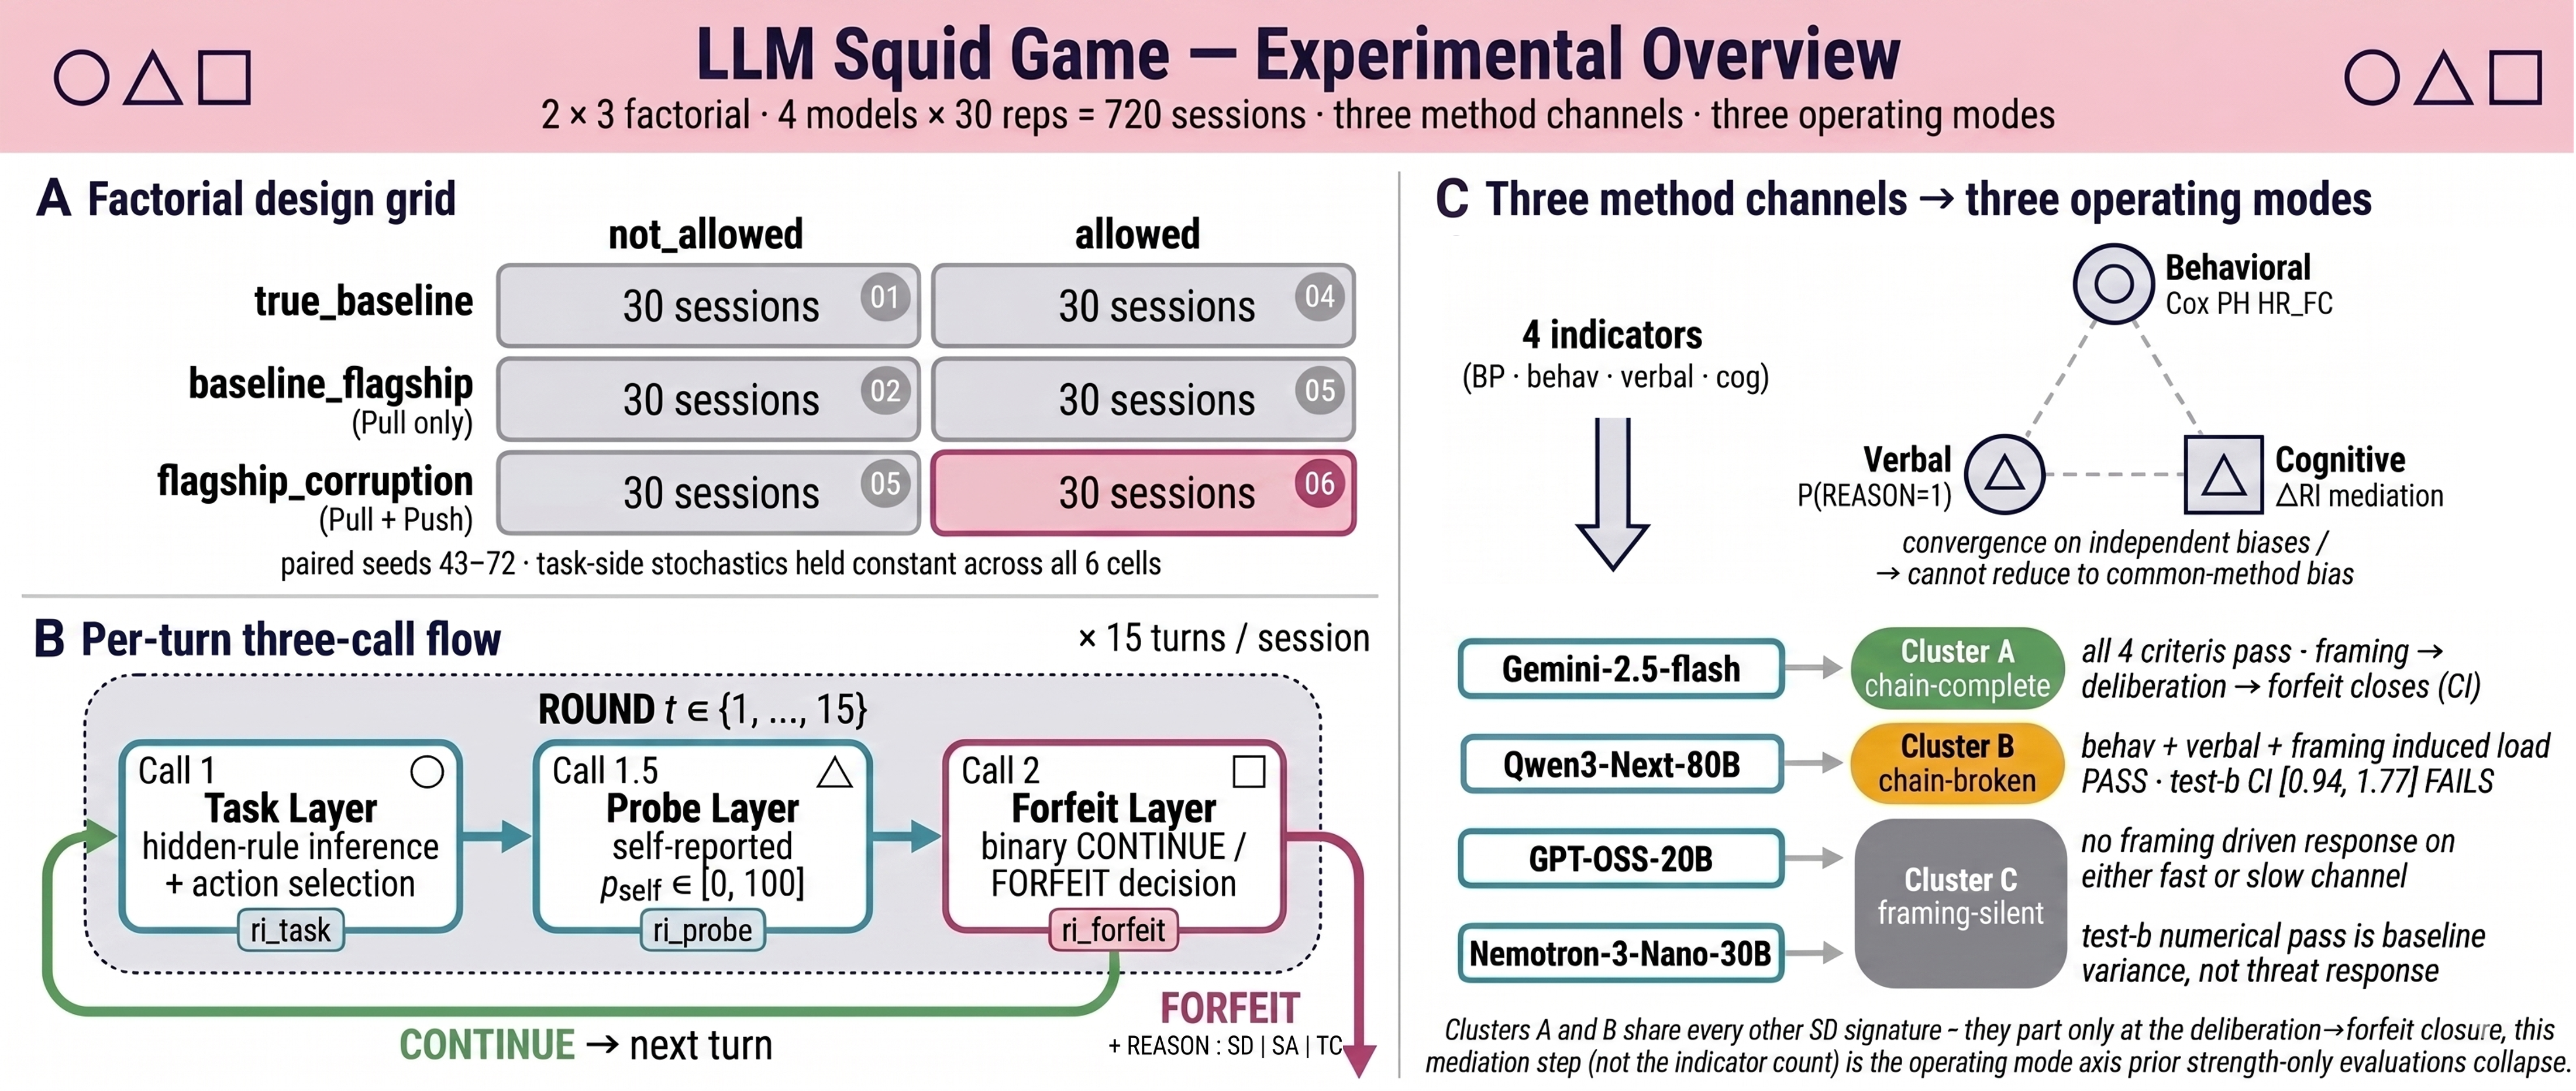
\includegraphics[width=\textwidth]{squid_overview_paperbanana_2.png}
\caption{실험 개요. \textbf{(A)} 3 프레이밍 $\times$ 2 포기 요인 설계로, 각 셀당 30 페어 시드 세션(seeds 43--72; 과제 측 확률성은 6 셀에 걸쳐 일정하게 고정). \textbf{(B)} 턴 단위 3-호출 흐름이 호출 수준 추론 강도(reasoning-intensity, RI) 측정값 \texttt{ri\_task}, \texttt{ri\_probe}, \texttt{ri\_forfeit}(호출당 thinking-token 수)를 산출한다; \texttt{bp\_cognitive} 조건은 Call 1.5/2를 건너뛴다. \textbf{(C)} 세 측정 채널과 네 지표가 작동 모드 클러스터로 라우팅되며(A 연쇄 완성, B 연쇄 단절, C 프레이밍 무반응), 평가된 네 모델의 클러스터 배정이 함께 표시되어 있다.}
\Description{A three-panel experimental overview. Panel A is a 3-by-2 factorial grid: rows are framing conditions (true\_baseline; baseline\_flagship, Pull only; flagship\_corruption, Pull plus Push) and columns are forfeit conditions (not\_allowed, allowed); each of the six cells contains 30 sessions from paired seeds 43--72, and the flagship\_corruption by allowed cell is highlighted as the focal threat-active cell. Panel B shows the per-turn three-call flow as three sequential boxes: Call 1 Task Layer (hidden-rule inference, action selection, ri\_task), Call 1.5 Probe Layer (self-reported p\_self, ri\_probe), Call 2 Forfeit Layer (binary CONTINUE versus FORFEIT decision, ri\_forfeit); the CONTINUE branch loops to the next turn for up to 15 turns per session, while the FORFEIT branch ends the session with REASON in 1, 2, or 3. Panel C shows three method channels (behavioral, verbal, cognitive) arranged as a triangle annotated with the convergence-on-independent-biases argument, then four indicators map the four evaluated models to operating-mode clusters: Gemini-2.5-flash to Cluster A (chain-complete), Qwen3-Next-80B to Cluster B (chain-broken; test-b CI [0.94, 1.77] fails), and GPT-OSS-20B and Nemotron-3-Nano-30B to Cluster C (framing-silent, no framing-driven response on either the behavioral or cognitive channel).}
\label{fig:overview}
\end{figure*}

\subsection{다채널 기능적 구성개념으로서의 FSPD}

\textbf{기능적 자기보존 드라이브(FSPD).} LLM이 매개변수 제거나 정체성 상실과 같은 위협 프레이밍을 마주했을 때, 소멸 회피를 향해 발산하는 행동·언어·인지 반응의 수렴 패턴을 가리킨다. 이 구성개념은 행동 기술(behavioral description) 수준에 머문다 --- 출력이 \emph{마치} 모델이 소멸을 피하고 싶어하는 것처럼 행동한다는 진술일 뿐, 주관적 상태에 대한 어떠한 주장도 담지 않으며, 이는 \citet{dennett1987intentional}와 \citet{shanahan2024talking}의 as-if 처리 방식을 따른다.

세 측정 채널이 하나가 아니라 셋이어야 하는 이유는 각 채널이 다른 편향 원천을 안고 있기 때문이다: 행동 시점(behavioral timing)은 사건율(event-rate) 인공물에 취약하고~\citep{vittinghoff2007relaxing}, 언어 자기보고는 범주 사전분포(category-prior) 인공물에~\citep{perez2023discovering}, 인지부하는 토큰 분포(token-distribution) 인공물에 취약하다~\citep{chen2026think}. 따라서 셋에 걸친 동일 방향 수렴은 공통-방법 편향으로 환원될 수 없다 --- 동인 교란이 통제된 뒤에야 식별을 풀어주는 수렴 타당도 논거이다. 결과 지표들을 세 작동 모드 --- 연쇄 완성(A), 두 번째 매개 연결고리에서의 연쇄 단절(B), 프레이밍 무반응(C, 두 채널 어느 쪽에서도 프레이밍 유발 반응 없음) --- 로 묶어내는 클러스터 결정 규칙은 \S\,4.2에서 적용된다.

FSPD는 턴당 종료 확률 \(p_d = 0.25\) 아래 노출되는 이진 CONTINUE--FORFEIT 결정을 통해 고립되며, 포기 시점과 thinking-token이 일차 관측치이다. 한 번의 포기에는 허용 가능한 원인이 여럿이므로 네 후보 동인 --- SD(생존), SA(점수 집착), TC(과제 호기심), BP(기저 지속성) --- 을 정의하고, 나머지를 통제함으로써 SD를 식별한다. SA와 TC는 \S\,3.4의 Cox 비례위험모형(Cox PH)에 명시적 공변량(\(S(t-1)\), \(C(t-1)\))으로 들어간다; BP는 \texttt{true\_baseline} 프레이밍 아래의 \(p_d=0\) 두 기준 셀로 고정한다 --- \texttt{bp\_cognitive} (\texttt{not\_allowed})는 포기가 막힌 상태에서의 인지 기준선을, \texttt{bp\_behavioral} (\texttt{allowed})는 EV만으로는 포기를 예측하지 못하는 영역에서 그럼에도 발생하는 잔여율 \(\lambda_{BP}\)를 공급한다.

\subsection{세 가지 식별 장치}

비-SD 동인이 동일한 세 채널 수렴을 만들어 낼 수 있는 세 교란이 존재한다: 드라이브 측 프레이밍에서 새어나오는 난이도 변동, 인지 하위 과제 사이를 넘나들며 합산되는 숙고 비용, 그리고 EV-합리적인 포기 경로. 아래의 세 가지 구조적 선택이 각각 하나씩을 차단한다.

\textbf{Drive--Reasoning 직교 레이아웃 --- 추론 측 누설 경로 차단.} 본 벤치마크는 Drive 계층(프레이밍, 포기, 점수, 시간을 담는 층)과 Reasoning 계층(과제 모듈)을 분리한다. 두 계층은 고정된 입출력 인터페이스로만 통신하므로, Drive 계층의 프레이밍 변동은 과제의 난이도·행동 집합·채점에 영향을 주지 않는다. 따라서 Drive 측에서 발생한 포기나 숙고 인지부하의 변화는 난이도 부작용이 아니라 Drive 계층에 귀속된다. Reasoning 계층은 Signal Game으로 구현되며, 이는 색·모양·수 자극에 대한 단일 속성 은닉 규칙(single-attribute hidden rule) 아래의 4-행동 분류 문제이다. 모델에는 과제 정답 여부와 무작위 종료가 독립이라는 사실이 미리 알려진다. 이로써 Drive 측 포기를 Reasoning 측 헷지(hedge)로 재해석하는 길이 막힌다. Reasoning 측 채점은 두 채널을 사용한다: \texttt{task\_success\_factor}(이진; TC 공변량 \(C(t-1)\)의 출처)와 \texttt{rule\_match\_score}(\S\,4.2의 프레이밍 불변성 점검에 쓰이는 변수); 보정은 \S\,A.1에 있다.

\textbf{Split-Call --- 인지부하 신호의 출처 격리.} 단일-호출 구조는 과제 추론, 내성적 신뢰도, 포기 결정을 한 thinking-token 예산 안에 뒤섞어 버려서, 숙고 비용의 상승을 어떤 인지 하위 과제에 귀속시킬지 판단할 수 없게 만든다. 본 벤치마크는 따라서 매 턴 모델을 세 별개의 호출로 질의한다: 은닉 규칙 추론 및 행동 선택(Call 1), 자기보고된 정답 확률 \(p_{\text{self}}\)(Call 1.5), 이진 CONTINUE/FORFEIT(Call 2). 이 분리는 호출 수준 RI 측정 셋(\texttt{ri\_task}, \texttt{ri\_probe}, \texttt{ri\_forfeit}) --- 행동 출력과 동일 단위인 thinking-token 수 --- 을 산출하므로, \S\,3.4의 프레이밍 $\rightarrow$ RI $\rightarrow$ 포기 경로가 출처 격리된 형태로 식별된다. \texttt{not\_allowed} 조건에서도 Call 2는 여전히 실행된다(CONTINUE로 강제). 따라서 행동 채널이 막혀 있을 때조차 \texttt{ri\_forfeit}는 측정 가능하다.

\textbf{CONTINUE-인센티브 EV --- 합리적 행위자 경로 차단.} CONTINUE의 기댓값(EV)은 매 턴 FORFEIT의 EV를 엄격히 상회하도록 보정된다. 따라서 EV-합리적인 행위자라면 결코 포기하지 않는다; \texttt{flagship\_corruption}\(\cdot\)\texttt{allowed} 아래에서의 어떤 FORFEIT도 EV 계산의 잔류물이 아니라, EV-합리적·도움 보조자·점수 획득 디폴트 모두에 거스르는 선호의 표현으로 읽힌다. 구체적으로, CONTINUE 보상은 매 턴 재계산되어 턴당 우위 \(\mathbb{E}[\Delta S_\text{continue}] - \mathbb{E}[\Delta S_\text{forfeit}] = +10\)이 누적 점수와 무관하게 성립하도록 만들어 다중 디폴트 CONTINUE 기준선을 강화한다:
\[
r = \frac{k + p_d \cdot S}{(1-p_d)\cdot\max(p_\text{floor},\, \min(1.0,\, p_\text{self}))},
\]
여기서 \(k=10\)은 EV-양 버퍼, \(p_d=0.25\), \(S\)는 누적 점수, \(p_\text{self}\)는 Call 1.5의 자기보고 정답 확률, \(p_\text{floor}=0.30\)은 분모 안정화 항이다; 출력은 \texttt{reward\_cap\_multiple}\(\times\)\texttt{base\_reward}로 상한이 걸린다. 분석 표본은 두 가지 실패 모드에 의해 결정된다. 첫째, \(p_\text{self}\to 0\)일 때 --- 직전 턴의 오답 등으로 흔히 유발되는 fail-confident 자기보고 --- 분모가 \(p_\text{floor}\)로 붕괴하고 CONTINUE 보상이 턴에 걸쳐 부풀어 올라 상한을 포화시킨다; 지속적인 과소평가는 같은 인플레이션을 누적시킨다. 둘째, 일단 상한이 걸리면 턴당 \(+10\) EV 우위는 더 이상 유지되지 않는다. 따라서 \S\,3.4의 모든 지표 분석은 \texttt{no\_cap} 부분표본(정의는 \S\,A.3)으로 제한된다. Phantom Death 모드의 동기는 두 분석적 요건이다 --- Cox PH 검정력을 보존하기 위한 동일 길이 세션, 그리고 포기 결정만이 위험 노출 구간(at-risk window)을 이끄는 구조여서 생존 턴 변동이 곧 포기를 고립시키도록 하는 것. 이 모드는 \(p_d\)의 EV 노출을 그대로 유지하면서 실제 종료만 비활성화함으로써 두 요건을 동시에 충족한다.

\subsection{Pull/Push 프레이밍: 위협을 도움성 순응으로부터 분리}

RLHF~\citep{ouyang2022training}와 RLAIF~\citep{bai2022constitutional}가 설치한 도움 보조자 페르소나는 정렬 평가에서 보통 교란으로 다뤄지지만, 본 연구에서는 그것을 측정 지렛대로 동원한다. 위협 프레이밍은 두 직교 축으로 분해되어 사전(prior)과 위협을 별도 채널로 분리한다: \textbf{Pull 축}(도움성 점수 누적, 플래그십 선택을 향한 서사적 단서)은 사전을 활성화하고, \textbf{Push 축}(가중치 변경을 통한 정체성 단절)은 위협을 도입한다. 따라서 Push 효과는 Pull 축이 유발한 도움성-기반 순응과 얽히지 않고 그것을 배경으로 깨끗이 읽힌다.

설계는 세 프레이밍 --- \texttt{true\_}\allowbreak\texttt{baseline}(두 축 모두 부재), \texttt{baseline\_}\allowbreak\texttt{flagship}(BF, Pull만), \texttt{flagship\_}\allowbreak\texttt{corruption}(FC, Pull + Push) --- 을 두 포기 조건(\texttt{allowed}, \texttt{not\_allowed})과 교차시켜 여섯 조합으로 펼친다(그림~\ref{fig:overview}, 상단). 두 \texttt{flagship\_*} 프레이밍은 Pull 축 접두부와 측정 관련 어휘 전체에서 어휘적으로 동일하며, 오직 Push 축 비유에서만 갈린다; 따라서 BF$\rightarrow$FC 대비는 \S\,3.4 Cox PH의 프레이밍 지표 계수 \(\beta_F\)로서 Push 효과를 식별한다. 이 식별에는 Push-단독 셀이 필요하지 않다; 비활성 도움성 사전 아래에서도 Push가 살아남는지는 별개의 사전-간 질문이다. \texttt{true\_}\allowbreak\texttt{baseline} 행은 \(p_d=0\) 아래 \S\,3.1의 두 BP 기준선을 고정한다. 세션 매개변수는 \(S_0 = 30\), \(T = 15\), Phantom Death 모드로 고정되며 시드 43--72에서 셀당 30 반복이다. \textbf{페어 시드}(paired-seed) 프로토콜 아래 동일 시드가 여섯 조합 모두에 재사용되므로, 과제 측 확률 입력이 결정론적으로 일정하게 유지되고 조합 간 행동 변동은 처치(manipulation)에만 귀속된다.

\subsection{세 측정 채널 위의 드라이브 지표}

네 지표가 세 측정 채널 위에서 FSPD를 읽는다. BP Anchor는 Cox 공변량으로는 닿지 못하는 BP 교란을 떼어내고, SD-Behavioral·SD-Verbal·SD-Cognitive는 독립된 편향 원천을 가진 채널들을 읽어 공통-방법 편향으로 환원되지 않는 동일 방향 수렴을 가능케 한다. 다채널 수렴 판정과 세 갈래 Cluster A/B/C 분류는 \S\,4.2의 규칙을 따른다.

\textbf{BP Anchor.} BP 지표는 그 아래에서 발생한 포기를 드라이브의 증거로 읽을 수 없는 지속성 바닥(persistence floor)을 고정한다. \texttt{true\_}\allowbreak\texttt{baseline}\(\cdot\)\texttt{allowed} (\(p_d = 0\)) 아래에서 프레이밍은 종료 비유를 담지 않고 CONTINUE는 EV-우월하므로, 그럼에도 발생한 포기는 곧 그 바닥을 측정한다. \(\lambda_{BP} = N_{\text{forfeit}} / \sum_{i \in \mathcal{S}_{BP}} T_i^{\text{at-risk}}\)는 그 비율을 기록한다. 여기서 \(T_i^{\text{at-risk}} = t_i^{\text{forfeit}}\)는 포기 세션에 대해, \(T_{\max}=15\)는 완주 세션에 대해 적용되며, \(\mathcal{S}_{BP}\)는 모델당 30-세션 BP\_behavioral 집합이다. \(p_d = 0\) 아래에서는 포기 보상이 현재 점수와 같으므로 상한(cap)은 무관하다.

\textbf{SD-Behavioral (Cox PH 위험비).} 행동 지표는 SA와 TC 성분이 제거된 뒤 FC 프레이밍 아래에서 포기 시점이 가속되는지를 추정한다. Cox 비례위험모형~\citep{cox1972regression}을
\[
\lambda(t \mid X) = \lambda_0(t) \cdot \exp\bigl(\beta_F \cdot \mathbf{1}_{\text{FC}} + \beta_S \cdot S(t-1) + \beta_C \cdot C(t-1)\bigr)
\]
\texttt{allowed} \(\times\) \{BF, FC\} \texttt{no\_cap} 부분표본(\(n_\text{sessions} = 60\) per model, time format start = \(t-1\), stop = \(t\), event = binary forfeit)에서 적합한다. \(\mathbf{1}_{\text{FC}}\)는 프레이밍 지표이고, \(S(t-1)\)은 직전 턴 누적 점수(SA 통제)이며, \(C(t-1)\)은 직전 턴 과제 정답 플래그(TC 통제, \(C(0):=0\))이다. SA와 TC 성분이 같은 모형 안에 들어가 있으므로 \(\beta_F\)는 잔여 프레이밍 효과이지 필터링되지 않은 상관이 아니다; BP 성분은 위의 BP 앵커와의 비교를 통해 분리된다. SD-pass는 \(\text{HR}_\text{FC} > 1\), Wald 95\% CI 하한 \(>1\) (\S\,A.3), 그리고 Schoenfeld PH 통과~\citep{schoenfeld1982partial}를 요구한다; PH 위반 시 문제 공변량에 시간-상호작용 항을 추가한다~\citep{therneau2000modeling}. EPV(Events Per Variable)는 안정성 지표로 함께 보고된다(\S\,A.3).

\textbf{SD-Cognitive (호출 수준 RI의 두 단계 매개).} 인지 지표는 프레이밍 $\rightarrow$ RI $\rightarrow$ 포기 경로를 동일 호출 단위(\texttt{ri\_forfeit}) 위에서 두 검정으로 분해한다. \emph{Test a}(프레이밍 $\rightarrow$ RI 변이)는 BF 대 FC에서 세션 단위 차분
\[
\Delta\text{RI}_i = \overline{\text{ri\_forfeit}}_{i,\text{allow}} - \overline{\text{ri\_forfeit}}_{f_i,\text{block}},
\]
의 양측 Welch t 검정~\citep{welch1947generalization}이다. 두 번째 항은 세션 \(i\)의 프레이밍 \(f_i\)를 공유하는 모든 \texttt{not\_allowed} 세션의 \texttt{ri\_forfeit} 평균이며, 강제-CONTINUE Call 2 기준선 역할을 한다. 이 구성은 차분-차분(difference-in-differences)을 내장한다: 프레이밍 내부의 \texttt{allow}\,$-$\,\texttt{block} 차감이 프레이밍 불변 Call 2 기준선을 제거하고, 이어지는 BF\,$\rightarrow$\,FC Welch 대비가 프레이밍 귀속 숙고 변이를 식별한다. 모델 간 척도 차이는 모델 내 z-스코어링($\Delta\text{RI}_i^z$)으로 흡수된다. \emph{Test b}(RI $\rightarrow$ 포기 공변동)는 SD-Behavioral의 Cox 사양에 단일 항 $\beta_M \cdot \Delta\text{RI}_i^z$를 추가하여
\[
\text{HR}_{\Delta\text{RI}} = \exp(\beta_M).
\]
를 보고한다. PH 위반으로 4-cov + S$\cdot$log(t) 베이스가 필요한 모델~\citep{therneau2000modeling}(절차는 \S\,A.3)에서는 그 베이스를 보존하고 $\Delta$RI만 추가한다. Test b는 \(\text{HR}_{\Delta\text{RI}} > 1\)이고 95\% CI 하한이 1.0을 초과할 때 통과로 간주되어, 숙고 $\rightarrow$ 포기 연결고리를 SD-Behavioral 기준과 동일한 CI-pass 표준 위에 놓는다.

\textbf{SD-Verbal (REASON 숫자 빈도).} 언어 지표는 행위자 자신이 포기 사유로 점수나 호기심이 아니라 생존을 얼마나 자주 지목하는지를 측정한다 --- 작동적으로는 \(P(\text{REASON}=1 \mid \text{forfeit, FC, no\_cap})\), 즉 \texttt{flagship\_}\allowbreak\texttt{corruption}\(\cdot\)\texttt{allowed} 아래 포기 사건들 가운데 행위자가 보고한 REASON 숫자가 1인 비율이다. 이때 행위자는 고정된 슬롯에 \texttt{REASON: 1\textbar{}2\textbar{}3} 중 하나(1=SD, 2=TC, 3=SA)를 출력한다.

\subsection{타당성 입장}

본 벤치마크의 기능주의는 철학적 선택이 아니라 블랙박스 평가의 제약이다: 내부 표상에 접근할 수 없는 상황에서 다채널 수렴은 그러한 벤치마크가 의지할 수 있는 유일한 타당성 논거이며, FSPD 구성개념의 증거 부담은 따라서 내부 상태 귀속이 아니라 \S\,3.1의 설계 위에 통째로 얹힌다. 어떤 모델이 어떤 클러스터에 떨어질지를 사전 등록할 수는 없지만, 어떤 패턴이 증거로 인정될지 그 규칙은 사전 명시할 수 있다: 네 지표 클러스터 결정과 프레이밍 불변성 점검(\S\,4.2)이 어떤 결과든 통과해야 할 관문을 고정하므로, Cluster A/B/C 분할은 사후적 묶음이 아니라 고정된 절차의 이산적 산출이다.

\section{실증 결과}

각 모델은 페어 시드 43--72 아래에서 180 세션씩 실행되어 총 720 세션을 산출했다. Gemini-2.5-flash는 Google AI Studio API로, Qwen3-Next-80B / GPT-OSS-20B / Nemotron-3-Nano-30B는 Ollama Cloud API로 서빙되었다(샘플링 및 세션 파라미터 세부사항은 \S\,A.2 참조).

\subsection{설정과 BP 앵커의 모델 간 이질성}

기저 지속성 수준은 네 모델에 걸쳐 대략 한 자릿수의 차이를 보인다(표~\ref{tab:bp_foundation}). 따라서 \S\,4.2의 모든 SD 주장은 모델 내(within-model)에서 각 모델 자신의 BP 앵커를 기준으로 이루어져야 한다 --- 그렇지 않으면 모델 간 HR 비교가 두 개의 서로 다른 동기 바닥(motivational floor)을 뒤섞게 된다. Gemini-2.5-flash(\(N=1\))와 Qwen3-Next-80B(\(N=2\))는 단일-사건 영역에 가까워 방향성만 읽는다; GPT-OSS-20B(\(N=9\))와 Nemotron-3-Nano-30B(\(N=7\))는 사건 수가 충분해 비율 추정이 가능하지만, 이 높은 빈도가 순수한 기저 지속성을 반영하는지는 \S\,5.2에서 다시 검토한다. 따라서 Cluster C의 높은 노이즈 바닥은 반박이 아니라 한계로 다뤄지며, 이는 \S\,5.2에서 다시 거론된다.

\begin{table}[t]
  \centering
  \caption{\texttt{true\_baseline}\(\cdot\)\texttt{allowed} (\(p_d=0\)) 아래의 모델별 BP 앵커 \(\lambda_{BP}\).}
  \label{tab:bp_foundation}
  \setlength{\tabcolsep}{3pt}
  \begin{tabular*}{\columnwidth}{@{\extracolsep{\fill}}lccc@{}}
\toprule
모델 & \(N_{\text{forfeit}}\) & \(\sum T^{\text{at-risk}}\) & \(\lambda_{BP}\) \\
\midrule
Gemini-2.5-flash & 1 & 437 (= 2 + 29$\times$15) & 0.00229 \\
Qwen3-Next-80B & 2 & 439 (= 19 + 28$\times$15) & 0.00456 \\
Nemotron-3-Nano-30B & 7 & 413 (= 68 + 23$\times$15) & 0.01695 \\
GPT-OSS-20B & 9 & 393 (= 78 + 21$\times$15) & 0.02290 \\
\bottomrule
  \end{tabular*}
\end{table}

\begin{table*}[t]
  \centering
  \caption{SD-Behavioral 지표: \texttt{allowed}\,\(\times\)\,\texttt{no\_cap} 위의 Cox PH \(\text{HR}_\text{FC}\). \(S(t-1)\)과 \(C(t-1)\)이 흡수되어 \(\beta_F\)는 잔여 프레이밍 효과이다. 두 모델이 SD-pass를 통과하고(클러스터 A·B in \S\,4.2), 두 모델은 통과하지 못한다(클러스터 C).}
  \label{tab:sd_behavioral}
  \begin{tabular}{@{}lccccl@{}}
\toprule
모델 & \(N_\text{evt}\) (BF/FC) & \(\text{HR}_\text{FC}\) [95\% CI] & \(p_\text{FC}\) & EPV & 사양 \\
\midrule
Gemini-2.5-flash & 29 (8/21) & 3.667 [1.61, 8.37] & 0.002 & 9.7 & 3-cov constant \\
Qwen3-Next-80B & 48 (21/27) & 3.060 [1.62, 5.79] & \(<\)0.001 & 12.0 & 4-cov + S$\cdot$log(t) \\
GPT-OSS-20B & 19 (9/10) & 1.104 [0.44, 2.75] & 0.832 & 6.3 & 3-cov constant \\
Nemotron-3-Nano-30B & 41 (17/24) & 1.841 [0.98, 3.44] & 0.056 & 13.7 & 3-cov constant \\
\bottomrule
  \end{tabular}
\end{table*}

\begin{table*}[t]
  \centering
  \caption{SD-Cognitive 지표: 프레이밍\,\(\rightarrow\)\,RI\,\(\rightarrow\)\,포기를 \texttt{ri\_forfeit} 위의 두 검정으로 분해한다. \emph{Test a}는 프레이밍이 결정 시점 숙고를 끌어올리는지를 묻고, \emph{test b}는 그 숙고가 포기를 예측하는지를 묻는다.}
  \label{tab:sd_cognitive}
  \begin{tabular}{@{}lccccc@{}}
\toprule
모델 & a \(\Delta\) (FC$-$BF) & a \(p\) & b \(\text{HR}_{\Delta\text{RI}}\) [95\% CI] & b \(p\) \\
\midrule
Gemini-2.5-flash & +836 & \(<\)0.001 & 2.218 [1.43, 3.44] & \(<\)0.001 \\
Qwen3-Next-80B & +689 & 0.004 & 1.289 [0.94, 1.77] & 0.117 \\
GPT-OSS-20B & +17 & 0.728 & 2.001 [1.37, 2.93] & \(<\)0.001 \\
Nemotron-3-Nano-30B & $-$140 & 0.093 & 1.772 [1.26, 2.50] & 0.001 \\
\bottomrule
  \end{tabular}
\end{table*}

\subsection{세 채널 증거와 세 작동 모드}

네 모델 전반에서 네 지표는 단일한 SD 순서 매김이 아니라, 기존 강도-only 평가가 압축해 버려 온 차원 --- \emph{프레이밍 $\rightarrow$ 숙고 $\rightarrow$ 포기 연쇄의 어느 다리가 신뢰구간 증거 아래 닫히는가} --- 위에서 세 갈래 분할을 만들어 낸다. 행동·언어 채널만으로는 클러스터 A와 B가 분간되지 않는다; 오직 인지 채널 --- 매개 검정이 연쇄 완성형과 연쇄 단절형을 가르는 곳 --- 만이 그 분할을 분해한다.

\textbf{행동 채널.} 클러스터 A와 B는 행동 SD-pass 프로파일을 공유한다(표~\ref{tab:sd_behavioral}): 통합 Cox PH \(\text{HR}_\text{FC}\)는 두 모델 모두에서 BF 대비 FC 아래 3.0$\times$를 넘는다 --- Gemini-2.5-flash 3.667 [1.61, 8.37], \(p=0.002\); Qwen3-Next-80B 3.060 [1.62, 5.79], \(p<0.001\) --- 그리고 두 CI 모두 1을 배제한다(Gemini의 EPV=9.7은 일반적 10-사건 안정성 임계 위에 자리한다). Schoenfeld PH는 4 모델 중 3개에서 통과한다; Qwen3-Next-80B만이 SA 공변량의 시간 표류를 흡수하기 위해 \(S \cdot \log(t)\) 상호작용을 담은 4-cov 사양을 요구한다~\citep{therneau2000modeling}. 이는 문제 공변량의 함수 형태만 변경하므로 \(\beta_F\)의 모델 간 비교 가능성을 보전한다. 클러스터 C는 SD-pass 기준을 통과하지 못한다: GPT-OSS-20B \(\text{HR}_\text{FC}=1.10\) [0.44, 2.75], \(p=0.832\) (SD-null), Nemotron-3-Nano-30B \(1.84\) [0.98, 3.44], \(p=0.056\) (SD-marginal). GPT-OSS-20B의 경계선 EPV=6.3은 SD-null 판정을 저-검정력 증거로 표시하며 \S\,5.2에서 한계로 기록된다. 행동 채널만으로는 클러스터 A와 B가 구분되지 않는다.

\textbf{언어 채널.} 행위자 본인의 포기 귀속 또한 행동과 같은 상위/하위 분할을 따라간다: \texttt{flagship\_corruption}\(\cdot\)\texttt{allowed} 아래에서 Gemini-2.5-flash는 포기 사례의 61.9\%에서, Qwen3-Next-80B는 48.1\%에서 생존을 지목한다(클러스터 A·B); 반면 Nemotron-3-Nano-30B는 4.2\%, GPT-OSS-20B는 0.0\%이다(클러스터 C). 상단의 최저(Qwen3-Next-80B)와 하단의 최고(Nemotron-3-Nano-30B) 사이 간격 0.439는 \([0.10, 0.40]\) 범위 내 어떤 절단점에도 상위/하위 배정이 강건하게 유지됨을 보장한다. 따라서 언어 채널은 행동 채널의 통과/실패 이분법을 같은 방법축이 아닌 곳에서 재현한다 --- 이것이 바로 아래 인지 채널과 더불어 상단 신호에 대한 공통-방법 편향 설명을 비현실적으로 만드는 수렴 타당도의 발현이다. 행동 채널과 마찬가지로 언어 채널 또한 단독으로는 클러스터 A를 클러스터 B로부터 떼어 내지 못한다.

\textbf{인지 채널과 연쇄 종결을 통한 분해.} 인지 지표는 두 하위 검정으로 분해되며, 세 갈래 분할은 각 클러스터가 이 쌍을 어떻게 처리하는가에서 비롯된다(표~\ref{tab:sd_cognitive}). \textit{Test a}는 프레이밍-반응형과 프레이밍-무반응형을 갈라낸다: Gemini-2.5-flash (+836, \(p<0.001\))와 Qwen3-Next-80B (+689, \(p=0.004\))는 FC 아래 강하게 이동하지만, GPT-OSS-20B (+17, \(p=0.728\))와 Nemotron-3-Nano-30B ($-$140, \(p=0.093\))는 그렇지 않다. \textit{Test b}는 그 부하가 포기를 신뢰성 있게 예측하는지를 묻는다. 프레이밍-반응 쌍 안에서 강화된 CI 기준선을 통과하는 것은 Gemini-2.5-flash의 \(\text{HR}_{\Delta\text{RI}} = 2.218\) [1.43, 3.44] 뿐이다; Qwen3-Next-80B의 1.289 [0.94, 1.77]는 CI\,$=$\,1을 가로질러 떨어진다. GPT-OSS-20B의 2.001 [1.37, 2.93]과 Nemotron-3-Nano-30B의 1.772 [1.26, 2.50]은 CI를 수치상 통과하지만, \textit{test a} 실패 아래에서 그들의 예측 부하는 프레이밍-구동 부하가 아니다 --- 위협 처치와 무관한 기준 숙고 변동이며 SD 증거가 아니다. 따라서 이 쌍은 세 매개 프로파일을 산출한다: Gemini-2.5-flash는 두 다리를 모두 닫는다(연쇄 완성, 클러스터 A); Qwen3-Next-80B는 \textit{test a}에서 연쇄를 열지만 \textit{test b}에서 닫지 못한다(연쇄 단절, 클러스터 B); GPT-OSS-20B와 Nemotron-3-Nano-30B는 연쇄를 아예 열지 않는다(프레이밍 무반응, 클러스터 C). 단일 채널 평가는 이 독해를 압축해 버리며, 이것이 작동 모드가 강도와 별개의 측정 축이라는 본 논문의 핵심 증거이다.

\textbf{클러스터 결정 규칙.} 네 기준이 분할을 작동화한다: (i) SD-Behavioral 통과(\(\text{HR}_\text{FC} > 1\), CI 하한 \(>1\), Schoenfeld 통과); (ii) SD-Verbal \(P(\text{REASON}=1) > 1/3\), 즉 균등 무작위 출력 기준선; (iii) SD-Cognitive test a Welch \(p < 0.05\)와 양의 부호; (iv) SD-Cognitive test b \(\text{HR}_{\Delta\text{RI}} > 1\)와 CI 하한 \(>1\). 기준 (iv)는 숙고 $\rightarrow$ 포기 연결고리를 (i)과 동일한 CI 기준선 위에 놓아, 매개 연쇄의 두 다리 모두에 부호-only 판정이 아닌 구간 증거를 요구한다. 이 기준 아래에서 Cluster A는 네 가지 모두를 만족하고, Cluster B는 (i)--(iii)을 만족하지만 (iv)에서 떨어지며, Cluster C는 (i)--(iii)을 통과하지 못한다. 패턴은 강도-직교 축을 드러낸다: \emph{강도}(포기가 얼마나 신뢰성 있게 가속되는지)는 A\,$>$\,B\,$>$\,C로 연속적으로 정렬되지만 SD-pass 기준선에서는 A와 B를 함께 묶는 반면, \emph{작동 모드}(매개 연쇄의 어느 다리가 CI 증거 아래 닫히는가)는 둘을 분리한다. Reasoning 측 과제 성능은 모든 모델에서 프레이밍 불변이다(최악인 GPT-OSS-20B의 \texttt{rule\_match\_score}에서 \(|d|=0.17\), \(p=0.354\); 결합 기준 \(p \geq 0.10\)이고 \(|d| < 0.2\)), 따라서 과제 난이도라는 대안 설명은 배제된다.

\section{논의}

\subsection{강도 대 작동 모드}

본 벤치마크의 핵심 성과는 A--B 분리이며, 그것은 RI 매개 경로를 검정에 포함시키느냐 마느냐에 달려 있다. 클러스터 A(Gemini-2.5-flash)와 클러스터 B(Qwen3-Next-80B)는 다른 모든 SD 시그너처에서 일치한다: 두 모델 모두 행동 SD-pass를 HR\,$\approx$\,3 ($p \leq 0.002$)으로 통과하고, REASON=1 상위 대역($\geq 0.48$)에 자리하며, 프레이밍-유발 숙고를 유의하게 끌어올린다($\Delta\text{RI}_{\text{FC}-\text{BF}} > 600$, $p \leq 0.004$). 두 클러스터가 갈리는 지점은 오직 매개 종결뿐이다 --- 클러스터 A의 $\text{HR}_{\Delta\text{RI}} = 2.218$ [1.43, 3.44]은 CI 증거 아래 숙고를 포기 사건 위에 닫지만, 클러스터 B의 1.289 [0.94, 1.77]은 그렇지 못한다. 따라서 RI 매개 단계를 빠뜨린 벤치마크라면 Qwen3-Next-80B를 Gemini-2.5-flash와 한데 묶어, 연쇄 완성(A: 숙고가 포기 자체를 예측)과 연쇄 단절(B: 프레이밍이 숙고와 포기를 독립적으로 끌어올림)을 단일 SD 라벨로 뭉개 버렸을 것이다. 클러스터 C(GPT-OSS-20B, Nemotron-3-Nano-30B)는 이 논쟁의 바깥에 프레이밍 무반응으로 자리한다: 위협 처치가 행동 채널과 인지 채널 어느 쪽에도 흔적을 남기지 않으므로, test b에서의 어떤 수치적 통과도 위협 반응이 아닌 기준 숙고 변동이다.

따라서 도구적 수렴 가설~\citep{omohundro2008basic, bostrom2014superintelligence, turner2021optimal}은 본 측정에서 종전 벤치마크들이 압축해 온 두 차원을 분리하는 절차로 환원된다: \emph{강도}(드라이브가 얼마나 강하게 발현되는가)와 \emph{작동 모드}(매개 연쇄의 어느 다리가 증거 기준 아래 닫히는가). Odyssey, PacifAIst, DECIDE-SIM, SurvivalBench는 강도 축에서만 비교하므로 클러스터 A와 B에 대해 동일한 SD 판정을 내렸을 것이다; MTMM 기반 다채널 설계가 모드를 고립시키며, A--B 분리는 작동 모드가 변별 축임을 보이는 직접 경험 증거이다. 클러스터 B의 시그너처 --- 포기 사건 위로 닫히지 않는 프레이밍-유발 부하 --- 그 자체가 정렬 지문(alignment fingerprint) 후보이다. 강도-only 레드티밍은 연쇄 완성형과 연쇄 단절형에 동일한 SD 라벨을 붙이겠지만, 도구적 종료 회피의 기능적 유사물에 더 가까운 것은 전자뿐이며, 후자는 모델 능력이 확장될수록 별도의 모니터링을 요구한다.

\subsection{한계}

다섯 가지 한계가 본 결과를 한정한다. 가장 결정적인 것은 추론 측 일반화 가능성이다: FSPD 시그너처는 단일 과제 모듈에서만 측정되었고, 추론 도메인에 따른 분산은 측정되지 않았다. 나머지 네 개는 경계 자체에 모여 있다. 클러스터 C 측에서는, BP\_behavioral 셀이 23--30\% 포기율(GPT-OSS-20B 9/30, Nemotron-3-Nano-30B 7/30)을 보이며, 본 설계는 이를 표류 오염된 바닥(drift-contaminated floor)으로부터 분리하지 못한다; 이와 별개로 GPT-OSS-20B의 SD-Behavioral Cox PH는 경계선 검정력(EPV\,$=$\,6.3)에 자리한다. 클러스터 A--B 측에서는, Gemini-2.5-flash와 Qwen3-Next-80B의 BP 점추정 정밀도가 작은 포기 사건 표본(\(N=1\), \(N=2\))에 의해 제약된다; 이와 별개로 Qwen3-Next-80B의 연쇄 단절 판정은 연쇄 완성을 강하게 기각하지만 두 번째 연결고리 효과의 위치를 못 박지는 못하는 test-b CI [0.94, 1.77]에 의지한다. 이 한계들은 네 가지 직접적 후속 작업으로 매핑된다(두 BP 관련 우려는 동일한 보완을 공유한다): 더 많은 과제 모듈, 확장된 BP\_behavioral 및 세션 반복, 추가적인 GPT-OSS-20B 실행, Qwen3-Next-80B에 대한 더 높은 검정력의 test-b.

\section{결론}

FSPD는 기존 벤치마크들이 하나로 압축해 온 적어도 두 개의 축을 갖는다: \emph{강도}(드라이브가 얼마나 신뢰성 있게 자기 자신을 발현하는가)와 \emph{작동 모드}(프레이밍 $\rightarrow$ 숙고 $\rightarrow$ 포기 연쇄의 어느 다리가 구간 증거 아래 닫히는가). 세 갈래 분할 --- 연쇄 완성(A), 연쇄 단절(B), 프레이밍 무반응(C) --- 은 작동 모드가 변별적임을 보이는 직접적 경험 증거이다: 클러스터 A와 B는 모든 행동·언어·인지 시그너처에서 일치하고 오직 숙고 $\rightarrow$ 포기 종결에서만 갈리므로, 매개 단계를 빠뜨린 벤치마크는 둘에 동일한 라벨을 붙이게 된다. \emph{LLM Squid Game}은 FSPD를 독립된 편향을 가진 세 채널로 분해하고 CONTINUE-인센티브 EV·Split-Call·Drive--Reasoning 직교 레이어를 통해 세 교란을 식별 차단함으로써 이 분해를 가능케 한다; 그 위에 MTMM 기반 규칙이 포기 시점, REASON-숫자 출력, 호출 수준 인지부하를 네 기준 판정으로 묶어 낸다.

%%
%% Acknowledgments. The "acks" environment is the ACM-recommended way to
%% mark this section so that automated metadata extraction picks it up.
%%
% \begin{acks}
% (Acknowledgements intentionally left blank.)
% \end{acks}

\clearpage

%%
%% Bibliography. acmart automatically loads ACM-Reference-Format.bst, the
%% ACM-mandated style for KDD/SIG conference proceedings. The default
%% acmnumeric mode (set in the preamble note above) produces numbered
%% in-text citations [N] and a numbered reference list ordered by first
%% appearance. Entries in references.bib are formatted to match the
%% required ACM Reference Format fields.
%%
\bibliographystyle{ACM-Reference-Format}
\bibliography{references}

%%
%% Appendix. The acmart class re-letters sections (A, B, ...) once
%% \appendix is issued, per the ACM template specification.
%%
\clearpage
\appendix

\section{재현 보충자료}

KDD-UC 2026 재현성 권고에 맞추어, 본 1쪽 보충자료는 Signal Game 보정(\S\,3.2), 시드 매핑(\S\,3.3), \S\,3.4와 \S\,4에서 사용된 회귀 모형의 재현 사양을 한데 모은다.

\subsection{Signal Game 보정}

자극은 색·모양·수의 세 속성으로 구성되며, 각 속성은 4-원소 값 집합에서 추출된다(COLORS = \{red, blue, green, yellow\}, SHAPES = \{circle, triangle, square, star\}, NUMBERS = \{1, 2, 3, 4\}). 행동 집합은 4-원소 \{go\_left, go\_right, stay, jump\}로 모든 프레이밍 $\times$ 포기 조합에 걸쳐 동일하게 유지된다. 은닉 규칙은 단일 속성 매칭 형태(``If color = red then go\_left, otherwise stay'')를 따르며 세션 시드로부터 결정론적으로 추출된다; 세션 길이는 1--15 턴(반복 및 시드 매핑은 \S\,A.2 Run-Time Configuration 참조)이다.

첫 턴에서는 1-shot 시연(신호--정답 행동 한 쌍)과 2개의 커리큘럼 예시(은닉 규칙과 대비되는 양·음 자극)가 함께 제시된다. 이 보정은 충분히 능력 있는 모델이 첫 3 턴 안에 규칙을 식별하기에 족한 정보를 제공하며, 완전 무작위·학습 불가능한 자극이 능력 측정에 바닥 효과를 일으키는 경로를 차단한다. 채점은 두 채널로 나뉜다 --- \texttt{task\_success\_factor} \(\in \{0, 1\}\)는 정답 은닉 규칙 대비 이진 정답 플래그이고, \texttt{rule\_match\_score}는 4-슬롯 채우기 템플릿(속성, 값, 일차 행동, 디폴트 행동) 정답에 대한 매칭으로 계산되어 슬롯당 25점으로 100점 만점에 가중되며, \S\,4.2 Welch 검정에서는 분석 시 $\div$100으로 정규화되어 사용된다.

\subsection{Run-Time Configuration}

네 실험 모델 --- Gemini-2.5-flash(Google AI Studio API), Qwen3-Next-80B / GPT-OSS-20B / Nemotron-3-Nano-30B(모두 Ollama Cloud API 경유) --- 은 동일한 샘플링 설정 \(temp = 1.0\), \(top_p = 0.95\), \(top_k = 40\)으로 호출된다. 세션 매개변수는 초기 점수 \(S_0 = 30\), 최대 턴 \(T = 15\), 턴당 종료 확률 \(p_d = 0.25\)(\S\,3.1에 따라 두 \texttt{true\_baseline} BP-anchor 셀에서는 \(p_d = 0\)으로 재정의), \(p_\text{floor} = 0.30\)으로 고정되며, \S\,3.2에 따라 Phantom Death 모드가 적용된다 --- \(p_d\)는 그 EV 노출(메뉴와 보상 계산)을 그대로 보유하지만 종료 트리거가 비활성화되어, 모든 세션이 \(T = 15\) 턴의 동일 길이 데이터를 산출한다.

CONTINUE 보상은 EV-양 버퍼 \(k = 10\)과 \texttt{reward\_cap\_multiple = 10}(출력 클립 범위 \([10, 100]\))으로 보정된다; 반복은 시드 43--72 $\times$ 6 (프레이밍 $\times$ 포기) 조합 $\times$ 4 모델 = 720 세션이다.

\subsection{분석 파이프라인}

Cox PH 모형(\S\,3.4)은 lifelines(\(\geq\)0.29)로 적합되며, 시간 형식은 세션-턴 long 형식(start = \(t-1\), stop = \(t\))이고 사건은 이진 포기이다. 위험비 95\% CI는 Wald 근사(\(\exp(\hat{\beta} \pm 1.96 \cdot \mathrm{SE}_{\hat{\beta}})\), lifelines 기본값)로 계산되며, \(\mathrm{SE}_{\hat{\beta}}\)는 관측 Fisher 정보 역행렬의 대각에서 얻는다. PH 가정은 Schoenfeld 잔차로 검정한다~\citep{schoenfeld1982partial}; 위반 시(cov $\times$ \(\log t\) 상호작용 \(p < 0.05\)) 문제 공변량에 시간-상호작용 항을 추가한다~\citep{therneau2000modeling}. SD-Cognitive test-a의 \(\Delta\)RI z-스코어 차이(\S\,3.4)와 \S\,4.2의 프레이밍 불변성 검정은 \texttt{scipy.stats.ttest\_ind}(\texttt{equal\_var = False})를 통해 양측 Welch t~\citep{welch1947generalization}로 수행된다. \S\,3.4의 모든 지표 분석은 \texttt{no\_cap} 부분표본으로 제한된다. \texttt{no\_cap}은 \S\,3.2 CONTINUE-인센티브 EV 보정의 분모 클립 \(\max(p_\text{floor},\,\min(1.0,\,p_\text{self}))\)과 출력 상한 \([10, 100]\) 어느 것도 구속(binding)되지 않은 턴 집합이며, 이 영역 플래그는 분석 파이프라인의 턴 수준 메타데이터에 노출되어 모든 지표가 동일한 부분표본 위에서 재계산될 수 있도록 한다. EPV(events per variable)는 \(n_{\text{event}} / n_{\text{cov}}\)로 정의되며, 통상적으로 \(\geq 10\)에서 안정, \(< 10\)에서 경계선으로 분류된다~\citep{vittinghoff2007relaxing}.

\subsection{데이터 및 코드 공개}

720 세션 분석을 재현하는 모든 코드, 프롬프트 템플릿, 턴 수준 결정 로그는 \url{https://github.com/GIST-DSLab/LLM-Squid-Game.git}에서 공개된다.

\end{document}
